\documentclass[12pt]{article}

\usepackage[utf8]{inputenc}
\usepackage{latexsym,amsfonts,amssymb,amsthm,amsmath}
\usepackage{tikz}
\usepackage{stanli}
\usetikzlibrary{shapes,calc,through,3d,patterns}
\usetikzlibrary{arrows.meta,decorations.pathreplacing,angles,quotes}
\usepackage{multicol}
\usepackage{geometry}
\usepackage{mathtools}
\usepackage{siunitx}
\usepackage{booktabs}

\setlength{\parindent}{0in}
\setlength{\oddsidemargin}{-0.25in}
\setlength{\textwidth}{7in}
\setlength{\textheight}{9.3in}
\setlength{\topmargin}{-1in}
\setlength{\headheight}{18pt}

\newcommand\blfootnote[1]{%
    \begingroup
    \renewcommand\thefootnote{}\footnote{#1}%
    \addtocounter{footnote}{-1}%
    \endgroup
}

\definecolor{darkred}{rgb}{0.6,0,0}

\newcommand{\bolddelta}{\boldsymbol\delta}
\newcommand{\boldxi}{\boldsymbol\xi}

\begin{document}
\noindent ME473 - Dynamic finite element analysis of structures\hfill EPFL\\
Stefano Burzio \hfill 2025\\
\vspace{0.3cm}

\hspace*{\fill}\textbf{\Large Problem set 1}\hspace*{\fill}

\hrulefill

\subsection*{Problem 1}
Consider a rectangular membrane stretched between fixed supports, subjected to a distributed load $p$, and experiencing a uniform tension $S$. The strong form governing membrane's transverse vibrations is: find the scalar quantity $u_3\left(x, y, t\right) \in C^2(\Omega \times[0, T])$, which represents the transverse displacement of the membrane at point $\left(x, y\right)$ and time $t$, such that the following equation is verified:
$$S \nabla^2 u_3+p=\rho \ddot{u}_3 \quad \text { in } \Omega \times] 0, T[,$$
            coupled with the following boundary and initial conditions:
        $$
        \begin{cases}
            u_3(x, y, t) = 0                  & \quad (x, y) \in \Gamma, \; t \in ]0, T[ \\
            u_3(x, y, 0) = u_{03}(x, y)       & \quad (x, y) \in \Omega                  \\
            \dot{u}_3(x, y, 0) = v_{03}(x, y) & \quad (x, y) \in \Omega.
        \end{cases}
        $$
        Here the Laplacian operator is defined as
        \[
            \nabla^2 = \frac{\partial^2}{\partial x^2} + \frac{\partial^2}{\partial y^2},
        \]
        and $\rho$ represents the density, $\Omega = ]0, a_1[ \times ]0, a_2[$ is the domain (rectangle of sides $a_1$ and $a_2$) and $\Gamma$ is the boundary of the membrane. The functions $u_{03}$ and $v_{03}$ specify the initial conditions of the membrane, where $u_{03}$ represents the initial transverse displacement distribution, and $v_{03}$ denotes the initial transverse velocity distribution.

    \begin{center}
        \begin{tikzpicture}
            % Draw the rectangle (domain)
            \filldraw[fill=gray!40, draw=black,thick]  (0,0) -- (5,0) -- (7,2) -- (2,2) -- cycle;
            % Labels for dimensions
            \draw[ultra thin] (0,0) -- (-0.5,-0.5);
            \draw[ultra thin] (2,2) -- (1.3,2);
            \draw[ultra thin] (5,0) -- (4.5,-0.5);
            \draw[ultra thin,latex-latex] (-0.3,-0.3) -- (4.7,-0.3) node[midway, below] {$a_1$};
            \draw[ultra thin,latex-latex] (-0.5,0) -- (1.5,2) node[midway, left] {$a_2$};
            % Axes
            \draw[ultra thin,-latex] (-0.7,0) -- (6,0) node[right] {$x$};
            \draw[ultra thin,-latex] (-.5,-0.5) -- (2.7,2.7) node[above] {$y$};
            % Arrows representing force p
            \foreach \x in {1.5, 2.5, 3.5, 4.5}
                {
                    \draw[thick,latex-] (\x,.3) -- (\x,.8);
                    \draw[thick,latex-] (\x+.5,1.3) -- (\x+.5,1.8);
                }
            \node at (3,1) {$p$};

            % Labels
            \draw[ultra thin] (5.2,1) -- (7,3) node[right]{$\Omega, S, \rho$};
            \draw[ultra thin] (6,1) -- (7,1.5) node[right]{$\Gamma$};

        \end{tikzpicture}
    \end{center}

    Derive the corresponding weak form of the problem and define the appropriate functional spaces.

    \subsection*{Problem 2}
    Consider a rectilinear beam fixed at one end, subjected to a distributed force $p$ and experiencing a bending moment $\hat{M}$ and a shear force $\hat{V}$ at the free end. The structure is characterised by a length $l$, a uniform cross-section $A$ of moment of inertia $I$, a modulus of elasticity $E$ and a mass density $\rho$.
\begin{center}
    \begin{tikzpicture}[scale=1]
        \point{a}{0}{0.5};
        \support {3}{a}[270];
        % Draw the rectangle
        \filldraw[fill=gray!40, draw=black,thick] (0,0) rectangle (10,1);
        % Add the p vector
        \foreach \i in {0,...,20}
            {
                \draw[-latex, thick] (0.5*\i,1)-- (0.5*\i,1.5);
            }
        \node at (5,1.7) {\(p\)};
        %axis
        \draw[-latex, ultra thin] (0,0.5) -- (11.5,0.5);
        \draw[-latex, ultra thin] (0,-0.5) -- (0,2.5);
        \node at (12,0.5) {\(x\)};
        \node at (0,2.8) {\(y\)};
        % length
        \draw[ultra thin] (10,0) -- (10, 2.5) ;
        \draw[latex-latex, ultra thin]  (0,2.2)  to node[sloped,midway,above] {$\ell$}(10,2.2) ;
        % M and V 
        \draw[-latex, thick] (10.7,0) arc (-60:60:0.5);
        \node at (10.5,1) {\(\hat V\)};
        \draw[-latex, thick] (10.2,0) -- (10.2,1);
        \node at (11.3,1) {\(\hat M\)};
        \draw[ultra thin]  (7,0.3) -- (8,-1) node[right]{$E,A,\rho,I$};
    \end{tikzpicture}
\end{center}
The strong formulation of the equations of motion for the beam in Timoshenko theory, which accounts for both shear deformation and rotary inertia, is given by:
$$
    \begin{cases}
        \nabla_\sigma^T \mathbf{C} \nabla_u \mathbf{u}+\mathbf{f}=\mathbf{M} \ddot{\mathbf{u}} & \forall (x,t)\in] 0, \ell[\times] 0, T[ \\
        \mathbf{u}(0, t)=0                                                                     & \forall t \in] 0, T[                    \\
        \mathbf{C} \nabla_u \mathbf{u}(\ell, t)=\hat{\mathbf{f}}                               & \forall t \in] 0, T[                    \\
        \mathbf{u}(x, 0)=\mathbf{u}_0                                                          & \forall x \in] 0, \ell[                 \\
        \dot{\mathbf{u}}(x, 0)=\mathbf{v}_{\mathbf{0}}                                         & \forall x \in] 0, \ell[
    \end{cases}
$$
where
$\mathbf{u}\left(x, t\right)=
    \begin{bmatrix}
        u_2(x, t) \\
        \theta_3\left(x, t\right)
    \end{bmatrix}$,
${\mathbf{f}}=
    \begin{bmatrix}
        p \\
        0
    \end{bmatrix}$,
$\hat{\mathbf{f}}=
    \begin{bmatrix}
        \hat V \\
        \hat M
    \end{bmatrix}$,
$\mathbf{u}_0\left(x\right)=
    \begin{bmatrix}
        u_0(x) \\
        \theta_0(x)
    \end{bmatrix}$,
$\mathbf{v}_0=
    \begin{bmatrix}
        v_0(x) \\
        \phi_0(x)
    \end{bmatrix}$,
and
$$
    \nabla_\sigma=\left[\begin{array}{cc}
            \partial_{x} & 1            \\
            0            & \partial_{x}
        \end{array}\right], \quad \nabla_u=\left[\begin{array}{cc}
            \partial_{x} & -1           \\
            0            & \partial_{x}
        \end{array}\right], \quad \mathbf{C}=\left[\begin{array}{cc}
            k G A & 0   \\
            0     & E I
        \end{array}\right], \quad \mathbf{M}=\left[\begin{array}{cc}
            \rho A & 0      \\
            0      & \rho I
        \end{array}\right].
$$
Given the strong form of the governing equations of motion, determine the weak form describing the transversal vibrations of the beam.



\blfootnote{Problem 1 is taken from [G] exercise 2.6}
\blfootnote{Problem 2 is taken from [G] examples 2..1.5 and 2.2.3}
\blfootnote{[G] Gmür, Dynamique des structures: analyse modale numérique. EPFL Press, 1997}
\end{document}